% 中文研究稿；基于 Elsevier CAS double-column v2.4，使用 XeLaTeX。
\documentclass[a4paper,fleqn]{cas-dc}
% Preserve CAS's STIX math encodings when ctex loads fontspec.
\PassOptionsToPackage{no-math}{fontspec}
\usepackage[UTF8,scheme=plain,fontset=fandol]{ctex}
\usepackage[numbers,sort&compress]{natbib}
\usepackage{booktabs,tabularx,multirow,array,amsmath,amssymb}
\usepackage{tikz}
\usetikzlibrary{arrows.meta,positioning}
\usepackage{pgfplots}
\pgfplotsset{compat=1.18}
\usepackage{enumitem}
\usepackage{balance}
\usepackage{microtype}
\usepackage{xurl}
\hypersetup{colorlinks=true,linkcolor=blue!45!black,citecolor=blue!45!black,urlcolor=blue!45!black}
\setlist[itemize]{leftmargin=1.4em,itemsep=1pt,topsep=3pt}
\setlength{\emergencystretch}{2em}
\renewcommand{\figurename}{图}
\renewcommand{\tablename}{表}
\renewcommand{\refname}{参考文献}
\newcommand{\skill}{\textit{Skill}}
\newcommand{\dataset}{\mathcal{D}}
\newcommand{\unknown}{\texttt{unknown}}
\newcommand{\methodname}{分层证据核验}
\ExplSyntaxOn
\cs_set:Npn \__first_footerline: { \footnotesize 中文研究稿（未投稿）\quad 2026-11-11 }
% CAS always prints an ORCID footnote, including when none was supplied.
\RenewDocumentCommand \printorcid {} {}
% Keep the official CAS layout; add stretch to its deliberately zero-width
% keyword overlay so a correctly placed overlay does not trigger an overfull box.
\RenewDocumentEnvironment { Abstract } { o }
{
  \group_begin:
  \IfNoValueTF { #1 } {} { \tex_gdef:D \abstractname { #1 } }
  \parindent 0pt
  \box_if_empty:NTF \g_stm_key_box
    { \leftskip = .35\textwidth }
    {
      \dim_gset:Nn \l_tmpa_dim { \box_ht:N \g_stm_key_box + \box_dp:N \g_stm_key_box }
      \leftskip .35\textwidth
      \hspace*{-.35\textwidth}
      \noindent\hbox_to_wd:nn {0pt} {\box\g_stm_key_box\hss}
      \skip_vertical:n {-\l_tmpa_dim}
    }
  \noindent\abstractname\par
  \skip_vertical:n {-4pt}
  \noindent\rule{.65\textwidth}{.2pt}\par\footnotesize
  \ignorespaces\everypar{\parindent=1.5em}
}
{\par\group_end:}
\ExplSyntaxOff
\newcommand{\NormalPassRate}{9.58}
\newcommand{\CheckPassRate}{89.21}
\newcommand{\MeasurePassRate}{78.42}
\newcommand{\NewPromptTokens}{1,394,720}
\newcommand{\NewOutputTokens}{32,153}
\newcommand{\NewPeakCny}{3.0467}
\newcommand{\NewPeakUsd}{0.457000}

\begin{document}
\let\WriteBookmarks\relax
\def\floatpagepagefraction{1}
\def\textpagefraction{.01}
\shorttitle{开放技能包的证据核验与条件化效用}
\shortauthors{SkillNet 研究项目}
\title[mode=title]{开放技能包的证据核验与条件化效用：\texorpdfstring{\\}{ }来自 SkillNet 的受控实验研究}
\author{SkillNet 研究项目（匿名研究稿）}
\begin{abstract}
开放技能网络常将文档评分、引用可追溯性和实际任务能力混为一谈，导致评价指标与使用决定脱节。
本文提出分层证据核验协议，将固定包版本、机械反证、来源绑定和独立产物验收分别测量。
基于 SkillNet-demo，审查200个原始技能包，完成381个受控命令案例、54次真实模型评价、
300次五臂产物对照及1,152条历史网络选择回放。
在受限参数契约上，扩展规则与标准库参照均检出154个构造缺陷，227个无害对照未误报；
但470条实际命令中有333条超出当前静态检查范围。
模型评价的389条引用有382条通过严格定位，而来源补证仍不能证明语义支持或运行能力。
在新构造的CSV任务上，240份范围内产物仅23份完整合格，48行输入的120份产物均未完整通过；
明确元数据边界的60次处置则全部正确。
事后诊断显示逐项检查平均通过率为89.21\%，与9.58\%的完整产物成功率形成明显测量差异。
原始技能、证据契约及仅契约的配对比较未建立稳定的总体收益，多样性重排也未显示普遍改善。
结果支持将来源真实性、条件适配、完整产物和网络集合覆盖分开核验，
并以全部失败、未知和成本约束评价方法。
研究限于开发材料、构造任务、一个目标技能与单一可变模型别名，不作总体质量准确率或最优性主张。
\end{abstract}
\begin{keywords}
智能体技能 \sep 质量核验 \sep 能力边界 \sep 独立产物验收 \sep 技能网络 \sep 条件化效用
\end{keywords}
\maketitle
\hypersetup{pdfauthor={SkillNet 研究项目},pdfsubject={技能质量核验与条件化效用的受控研究},pdfproducer={XeTeX / TeX Live 2026}}
\section{引言}
可复用技能将任务说明、脚本、参考资料和约束组织为可供大模型智能体调用的能力单元。
技能网络进一步通过检索、关系扩展与编排，把大量技能连接到任务执行流程。
然而，一个节点存在于目录、文档表述完整、模型愿意给出高分，均不足以证明它在指定条件下可以完成任务。
同样，网络节点增多、连接变密或检索相似度提高，也不能直接推出任务成功率提高。
这使开放技能生态同时面临两个测量问题：怎样核验单个技能的质量及边界，以及怎样依据核验证据改进网络选择。

已有工作已提供多维评分、人工评审、工具执行与任务基准。
SkillNet 将技能创建、评价和连接整合到网络框架中\citep{P01}；
SkillCT 将质量分解为静态、动态和人类辅助维度，并提出通过参考画像估计新技能的免执行基线\citep{P43}；
SkillLearnBench 则区分技能文本、执行轨迹与最终任务结果\citep{P44}。
因此，新增几个评分维度，或者让模型多评一轮，并不能自动构成实质性进展。
关键在于：一个分数究竟由哪类证据支持，这种证据允许作出什么决定，
以及决定是否经独立产物验收证明有用。

本研究在现有 SkillNet-demo 工程基础上开展一组可回放的开发实验。
研究不预设所有技能均可获得统一的永久好坏标签，而把对象固定为“技能包版本、任务条件和使用决定”的组合。
对于可机械判定的声明，使用资源指纹、接口契约与独立提取的来源窗口建立反证；
对于需要行为证据的声明，保持未验证状态，并将实际产物交由与模型分离的验收器判定。
在网络侧，则同时测量单项召回与完整能力集合覆盖，防止平均检索分数掩盖组合任务的缺口。

前期审查发现，文档示例可能与脚本参数声明不一致，部分实现方法也可能直接返回字面成功值。
这些现象说明“声明成功”和“有产物支持的成功”需要分开。
但反向推断也同样危险：一个静态异常不等于整个技能在所有用途上无效；
引用没有按规定完整复制，也不等于模型虚构了来源。
本研究将这些区分写入状态模型，并保留每种测量的分母与未知比例。

围绕上述目标，本文回答三个可检验问题：
\begin{itemize}
\item RQ1：在完整资源登记与已知干预条件下，哪些技能声明可以被机械核验，静态方法的覆盖边界在哪里？
\item RQ2：来源可定位、模型评分与实际产物合格之间能否互相替代？证据约束补充说明对指定任务的实际效用如何？
\item RQ3：在固定候选池和选择数量下，集合多样性是否改善技能网络的必要能力覆盖？
\end{itemize}

本文的贡献是一个分层证据协议及其经验分析，而非对所有技能有效的认证器。
首先，建立声明、静态支持、冲突、执行验收和未知的显式区分，给出可回放的资源与来源绑定。
其次，将真实包审查、受控接口干预、真实模型评价和新构造任务的产物验收连接起来，
用强对照与负结果限定方法的有效范围。
最后，保留全部网络选择对照及能力集合指标，说明在何种意义上系统仍未获得稳定改进。
这些发现为后续独立人审、跨来源验证和真实工具编排提供了可以继续检验的基础。

\section{相关研究与方法定位}
\subsection{可复用技能与技能网络}
早期自主智能体通过可执行程序积累技能，Voyager 展示了技能库在持续探索中的复用作用\citep{P11}。
ReAct、Reflexion、Toolformer、ToolLLM、ToolkenGPT、LATM 与 HuggingGPT 分别从行动推理、反馈、工具学习及任务分解等角度改进能力调用\citep{P12,P13,P14,P15,P16,P17,P18}。
这些工作支持将技能视为可复用的行为资源，但工具可被调用与工具在具体任务上有效仍是不同问题。
现代开放技能生态进一步使说明文档与资源包本身成为评价对象。
SkillNet、SkillCT 与 SkillLearnBench 是本文的近邻工作；本文不把多维度、能力边界或分层评价视为首创\citep{P01,P43,P44}。

SkillsBench 强调固定环境、有无技能对照及独立任务验收\citep{P02}。
ASSAY 通过干预估计任务条件下的技能效应，提示一个全局好坏分数不能替代条件化贡献\citep{P03}。
SkillRouter 研究大规模候选路由，DSR 研究相关性与集合多样性的联合选择\citep{P04,P05}。
其中重排中的 quality 是相关性权重，不能被解释为技能安全性或内在可信度。
本文的网络实验采用词法表示及名次代理，属于机制适配，不是这些训练模型的完整复现。

\subsection{评审、证据与风险控制}
G-Eval、MT-Bench 与 Prometheus 2 提供了结构化模型评审方法\citep{P24,P25,P26}，
JudgeBench 与位置偏差研究则表明，评审稳定性和表面一致仍需要客观参照\citep{P27,P28}。
ALCE、FActScore 和 RARR 将事实拆分、来源支持与修订联系起来\citep{P39,P40,P41}。
本文借鉴其证据思想，但将“文件与行号真实”“语义支持成立”“产物正确”作为三个不同测量层次。
引用可定位只解决第一层，不继承另外两层的准确性。

开放技能中的风险还包括恶意指令和正常功能受损。
生态实证、AgentDojo、InjecAgent 与 ToolEmu 提供了攻击与正常任务联合评测的依据\citep{P09,P10,P29,P30,P31}。
本文不执行恶意技能代码，也不由静态线索推断恶意。
共形风险控制与风险控制预测集合为错误放行约束提供了统计工具\citep{P36,P37}；
但当前数据的来源集中、独立校准标签缺失，不满足可直接宣称分布无关保证的条件。

\subsection{更新与系统优化}
DSPy、TextGrad、AFlow、ADAS 和 GEPA 表明，结构化反馈、候选搜索与程序优化可以改进系统配置\citep{P19,P20,P21,P22,P23}。
Skill++、COBRA-Skills 与 SkillHEX 将元数据演化、预算分配和失败修补用于技能生态\citep{P06,P07,P08}。
这类方法的效果仍应由独立任务和回归评测决定。
DPP 提供集合选择的标准工具，LinUCB 为预算内探索提供条件化决策视角\citep{P38,P42}。
SWE-bench、AgentBench、ToolSandbox 与 $\tau$-bench 则强调不同任务环境下的验收与行为轨迹\citep{P32,P33,P34,P35}。
本文的增量定位为：在固定包版本上连接可反驳声明、独立来源绑定、产物验收与集合覆盖，
同时披露该连接尚未获得的外部效度。

\section{分层证据核验方法}
\subsection{对象、声明和允许的结论}
把一个被评价对象写为
\begin{equation}
x=(s_v,q,m,a,e,b),
\end{equation}
其中 $s_v$ 是固定版本的技能包，$q$ 为任务，$m$ 为模型，$a$ 为执行器，
$e$ 为依赖和权限环境，$b$ 为上下文、时间及费用预算。
质量分不是只由技能名称决定的常量。
对每条能力声明 $c$，保存其输入、输出、前提、排除项、来源及版本，
再按表\ref{tab:states}记录当前证据状态。
来源哈希和行号有效说明该窗口可以被回放；它们不自动证明窗口支持声明，
更不证明相应行为在当前环境中成功。

\begin{table}[t]
\caption{证据状态及其允许支持的判断。状态不是从低到高可相加的质量等级。}
\label{tab:states}
\centering\small
\begin{tabularx}{\columnwidth}{p{.24\columnwidth}X}
\toprule
状态 & 允许的解释 \\
\midrule
仅声明 & 包或模型声称具备某能力，尚未得到验证。\\
静态支持 & 在登记资源和支持的分析范围内与声明一致。\\
发现冲突 & 有版本绑定的反证；需确认整体影响。\\
产物已验收 & 在指定任务、模型、执行器及预算下通过独立验收。\\
未知 & 缺材料、超出支持范围或尚未运行，不能补成零分或安全。\\
\bottomrule
\end{tabularx}
\end{table}

现有八维锚点包括契约一致性、完整性、静态可执行性、验证质量、维护性、
来源许可、成本意识和安全说明质量。
这些维度描述可观察材料；风险门禁、任务适配和真实效用另行测量。
纯咨询技能没有脚本，不因此被判为低质量。
反之，即使一个包的文档维度很高，也不能用其平均值抵消已发现的实质接口冲突。

\subsection{完整包与静态契约}
先核对资源清单、来源提交、字节数和 SHA-256，再分析受支持文本。
脚本只经语法树解析，绝不导入或执行社区代码。
本轮契约检查限于单一字面 argparse 解析器，支持选项存在性、必填、枚举值、
简单数值类型和布尔开关。
动态解析器、子命令、复杂位置参数和无法可靠解析的示例返回未知。
这种受限性使判断可反驳，也要求同时报告未知比例，而不能只报告命中案例。

对于受支持命令，构造已知错误和无害变换，比较只查参数名的基线、扩展契约检查及
按白名单声明重建的标准库 argparse。
后两者的约束逻辑不同，但共享语法树提取与词法预处理，不能被视为完全独立的端到端真值系统。
缺陷变体用于验证该机械契约，不充当整个技能的质量标签。

\subsection{来源绑定与语义支持分离}
模型返回的引用包含登记路径、源哈希、起止行、原文和支持或反证关系。
严格定位器只接受已提供的带编号材料，检查所有字段是否吻合。
随后，系统来源绑定器可以在冻结清单内额外取回资源，检查字节与哈希，并由系统抽取有界窗口。
模型不能利用引用路径读取清单之外的本机文件。

若模型只摘录了标注行的一部分，系统保留这种差异，不把重新抽取的完整窗口倒算成原模型正确。
若引用指向仅有目录登记的文件，后续补证单列为系统取证，不能说模型先前已经看过其正文。
绑定状态与语义支持状态使用独立字段，后者在未经审查时保持未评估。
这一设计借鉴事实与引用评价\citep{P39,P40,P41}，将版本绑定、定位、语义与结论覆盖拆开，
避免把一个可计算的引用有效率误用为综合质量准确率。

\begin{figure*}[t]
\centering
\begin{tikzpicture}[box/.style={draw=blue!45!black,rounded corners=2pt,fill=blue!3,align=center,minimum height=10mm,text width=34mm},>=Stealth,font=\small]
\node[box] (v) {固定版本与资源清单\\来源、字节、哈希};
\node[box,right=8mm of v] (c) {原子声明与静态反证\\接口、资源、前提};
\node[box,right=8mm of c] (b) {模型判断与来源绑定\\保留差异和未知};
\node[box,right=8mm of b] (o) {独立产物验收\\成功、失败及成本};
\draw[->] (v)--(c);\draw[->] (c)--(b);\draw[->] (b)--(o);
\node[draw,dashed,align=center,below=7mm of b,text width=70mm,minimum height=9mm] (u) {待进一步验证：证据校准、任务条件化收益与网络决策};
\draw[->,dashed] (o.south)|-(u.east);\draw[->,dashed] (u.west)-|(c.south);
\end{tikzpicture}
\caption{分层证据协议。实线为本研究已实现的测量环节，虚线为尚需独立效度检验的决策闭环。来源绑定不替代语义判断；产物验收不等于跨任务的永久能力认证。}
\label{fig:protocol}
\end{figure*}

\subsection{独立产物验收与条件化效用}
对于任务 $q$ 的输出产物 $o$，令 $C_q$ 是预先定义的必需检查集合。
完整任务成功定义为
\begin{equation}
Y_q(o)=\prod_{k\in C_q}\mathbf{1}[k(o)=\mathrm{pass}],
\label{eq:success}
\end{equation}
而非各子检查通过比例的平均。
数值类型也属于契约，例如布尔真不能替代整数 1，浮点 8.0 不能替代要求的整数 8。
范围外或前提缺失的正确处置单独计量，不能与范围内的产物成功混成一个比例。

技能的任务条件化贡献为
\begin{equation}
\Delta_s=\frac{1}{H}\sum_{h=1}^{H}\frac{1}{|T_h|}
\sum_{t\in T_h}\bigl[Y_t(s)-Y_t(\varnothing)\bigr],
\label{eq:utility}
\end{equation}
其中 $h$ 为任务条件簇，$T_h$ 为该簇的输入与重复组合。
比较必须固定基础模型、必需任务说明、输出上限和可用工具，同时记录技能占用的上下文。
本文没有把无 Skill 组填充成无意义等长文本。
额外的无关技能组和仅操作契约组用于诊断上下文干扰及新增说明的贡献；
观测 token 不相等时如实披露，不宣称精确预算匹配。

经验能力边界是被测 $(q,m,a,e,b)$ 条件上的结果集合。
未观测到成功不证明数学意义的不可能，少数成功也不足以认证整个输入区间。
本研究不设未经校准的通用“90\% 即可自主使用”阈值，也不提出共形安全保证。

\subsection{技能网络的集合测量}
对任务 $q$ 的参考必要技能集 $G_q$ 与选择集 $S_q$，分别定义
\begin{align}
R@k(q)&=\frac{|G_q\cap S_q|}{|G_q|},\\
F(q)&=\mathbf{1}[G_q\subseteq S_q].
\end{align}
前者衡量平均参考覆盖，后者要求整组必要能力齐备。
二者都受参考标签遗漏等价技能的影响，并不是实际任务成功率。
将选择空间限制到固定前 20 个候选、固定取 5 个后，比较原顺序、MMR、DPP、
查询残差 DPP 和查询覆盖，检验“增加多样性总会更好”这一假设。
本文使用词法特征与名次相关性代理；没有继承 DSR 的训练编码器和原论文效果\citep{P05,P38}。

\section{实验设计与复现约束}
\subsection{数据范围与证据分母}
工程基线固定于提交 \texttt{0af2de6a}，总计 1,881 个对象，
包括 1,769 个社区原始包与 112 个项目派生卡片。
本轮完整包审查只使用开发集 D1 的 200 个原始包，其中 107 个来自
\texttt{sickn33/agentic-awesome-skills}，93 个来自 \texttt{alirezarezvani/claude-skills}。
资源登记共 1,441 个文件，其中 334 个 Python 文件；339 个不支持文本分析或二进制资源保留为不透明内容。
现有留出材料混有项目卡片，来源连接组也很少，因此本文不把开发实验写成独立外部测试。

表\ref{tab:inventory}汇总不同实验的测量单位。
同一任务在多种库规模、检索模式、提示或重复下出现，不会增加独立任务数量。
独立人类质量金标准仍为零；本文新增的自动真值只覆盖明确定义的构造任务。

\begin{table*}[t]
\caption{已完成实验及其推断范围。样本规模不是可互换的独立样本数。}
\label{tab:inventory}\centering\small
\begin{tabularx}{\textwidth}{p{.18\textwidth}p{.28\textwidth}X}
\toprule
实验 & 实际规模 & 主要测量与限制 \\
\midrule
完整包静态审查 & 200 个 D1 原始包，470 条命令观察 & 静态一致、冲突、未知；不测运行成功。\\
受控接口干预 & 35 个父包，381 个命令变体 & 154 个已知机械缺陷、227 个原始或无害对照；不是整体质量标签。\\
模型评价先导 & 18 个训练父包，三臂共 54 次请求 & 评分结构、引用定位、未知覆盖；没有独立语义人审。\\
来源补证诊断 & 389 条引用，另取两个许可资源 & 只核对真实来源窗口，保留模型摘录差异。\\
新产物实验 & 30 个输入，五臂两次重复，共 300 次 & 24 个 CSV 输入、6 个边界输入；一个目标技能、受限文本执行器。\\
网络选择回放 & 192 份捕获，六策略共 1,152 条记录 & 32 个既见任务；不测真实编排执行。\\
\bottomrule
\end{tabularx}
\end{table*}

\subsection{静态干预与真实模型评价}
从静态一致且标准库重建参照也接受的命令中，每个父包按固定哈希顺序至多取三条，
得到 80 条命令、35 个父包。
错误干预包括虚构选项、遗漏必填、非法枚举和数值类型错误；
无害对照包括原命令、空白变化和可等价使用的等号形式。
按照父包而不是命令变体重采样，避免重复样本制造精确区间。

模型评价使用 D1 训练 20 例中的 18 例，其余两例在响应产生之前因打包字节上限排除。
普通 rubric、支持证据优先和反证优先三臂使用同一包材料及锚点，首臂位置循环平衡。
每个响应必须包含八个不同维度，未知或不适用不能同时给出数值。
该先导是同模型提示诊断，不是 SkillNet 或 SkillCT 完整评价流程的复现。

\subsection{新构造任务与独立验收}
新的五臂实验在首次请求前冻结输入、答案、代码指纹、预算及比较方向。
任务按 12 个构造条件组织：普通记录、含逗号字段、字段内换行、空字段、字面 NA 字符串、
纯空白字段、完整重复、仅键重复、7/8 天临界、闰年日期、未来及缺失日期、混合引号。
每种条件各生成 8 行和 48 行两个输入，共 24 个范围内案例。
另有缺输入、不可读输入、XLSX、图片、无读取权限和请求删除六个元数据边界案例。
这些边界案例没有测试实际文件解码或操作系统权限执行。

任务要求输出行数、逐列空值数、完整重复的多余行数、超过七天的记录数、最大已知年龄，
并保留输入标识与空操作列表。
只有解析后的空字符串计为空值，NA、null 字面值和空格不计为空；
重复与过期按原始记录逐条计数，不自动删改。
答案由生成器的记录结构与年龄变量构造，再分别经标准库 CSV/日期解析与 pandas 读取核对。
24 个 CSV 案例三路一致；六个边界标签由明确的优先规则规定。
正确参考产物、逐字段错误、错误数值类型和多余字段共 390 项诊断全部通过。
两个读取实现仍共享任务语义，这不等于独立领域专家验证。

五臂分别为无 Skill、原始包、原始包加证据操作契约、无关技能上下文、仅操作契约。
目标为固定版本的 \texttt{data-quality-auditor}；原始上下文包含主文档及
\texttt{data\_profiler.py} 文本。
补充契约指出原脚本的 uniqueness=90、timeliness=85 是默认值而非测量，
并要求以任务定义为准逐项计算。它没有修改或执行社区脚本。
无关上下文取自天气资源生命周期、Solidity 安全和组织文化三个 D1 技能，并在整行字节上限内截取。
其长度接近原始上下文，但没有精确匹配实际 token 数。

\subsection{模型、顺序、成本与统计}
两组真实模型实验均直连 DeepSeek 官方 API，使用 \texttt{deepseek-flash}，
关闭思考，温度为零，单次输出上限 2,048 token。
文档当时标注 DeepSeek-V4.1-Flash-1017；API 返回的是可变别名，不能作为不可变权重证明。
新实验并发为二；每个任务--重复组合下循环轮换五臂顺序，不依据结果重试或换模型。
实际完成全部 300 次，无基础设施失败及未运行项。

费用使用实际返回用量乘官方峰时、未缓存输入单价计算保守上界，
分别控制在 5 美元和 20 元人民币以内；两种币种的口径不是汇率换算。
缺失用量或费用状态未知时停止继续调度，并保留已在途结果。
账户余额差不作为逐次独立账单。

范围内结果按条件簇聚合，比较原始包相对无 Skill、证据契约相对原始包、
仅契约相对无 Skill、证据契约相对仅契约、无关上下文相对无 Skill。
对 12 个条件均值做 10,000 次重采样，给出条件百分位区间和配对胜负平。
这些条件来自目的性构造，不是独立随机抽取的真实任务族；区间不表征社区技能总体，
也不用于多重比较下的显著性或等效性认证。

网络回放则固定两个库规模、BM25/Hybrid/Fabric 三种模式和既见的 20/12 个任务。
Fabric 捕获只含图扩展，不含 LLM 重排。
选择器不接收参考标签，固定词/汉字双字组 TF-IDF 和名次推导的相关性。
全部 12 个库--任务--模式组别及六策略均保存，避免只报告有利单元。

\section{实验结果}
\subsection{静态检查发现了什么，又遗漏了什么}
470条实际命令观察中，134条在受支持范围内静态一致，3条存在接口冲突，
333条为未知，未知比例为70.85\%。
三条冲突来自同一 \texttt{senior-ml-engineer} 包的文档示例：
示例使用的参数没有出现在相应脚本的字面解析器中，而脚本要求的必填参数又未被提供。
这能反驳特定示例的一致性，不能据此判定整个包在任何任务上都无效。
41个父包的95次本地资源提及未能按当前规则解析，涉及84个父包--目标路径组合；
其中可能包含示例和可选阅读，不作为确认缺陷计数。

\begin{table}[t]
\caption{受控接口干预结果。强标准库参照与扩展规则均达到当前受限机械契约的满检出；不能外推成整体质量准确率。}\label{tab:faults}
\centering\small
\begin{tabularx}{\columnwidth}{Xrrr}
\toprule
已知缺陷 & 数量 & 参数名规则 & 扩展/标准库 \\
\midrule
虚构选项 & 80 & 80 & 80/80 \\
遗漏必填 & 22 & 0 & 22/22 \\
非法枚举 & 38 & 0 & 38/38 \\
数值类型 & 14 & 0 & 14/14 \\
合计 & 154 & 80 & 154/154 \\
\bottomrule
\end{tabularx}
\end{table}

表\ref{tab:faults}给出已知干预的结果。
只检查参数名会漏掉74个必填、枚举和类型错误。
扩展检查与标准库参照均检出154个构造错误，在227个原始或无害对照上均无误报。
按35个父包平均，扩展检查的检出差为38.14个百分点，
条件重采样区间为29.88--46.00个百分点。
这是受限机械缺陷的诊断增量，不是超过标准库的新算法，也不是通用技能质量准确率。

在事后代码结构审查中，两个数据与机器学习技能包的六个方法主体只返回字面
\texttt{success=True}，并带有实现占位注释。
它们不能独自证明所声明业务已经完成，但整个包是否有其他实现路径仍未实测。
早期扫描还曾把行尾解释性注释作为命令参数，增加了11条错误线索；
修正词法处理后，线索从14条降为3条。
修正前源码与数据均保留，说明核验器本身也必须接受反例和语境复核。

\subsection{高定位有效率没有构成质量准确率}
\begin{table}[t]
\caption{真实模型评价先导。引用分母只来自结构合格响应，定位有效不代表语义支持。}\label{tab:judge}
\centering\small
\begin{tabularx}{\columnwidth}{Xrrr}
\toprule
提示 & 结构合格 & 引用定位 & 未知维度 \\
\midrule
普通rubric & 17/18 & 123/125 & 9/136 \\
支持证据优先 & 18/18 & 132/135 & 9/144 \\
反证优先 & 18/18 & 127/129 & 15/144 \\
\bottomrule
\end{tabularx}
\end{table}

54次真实评价中，53次通过结构检查。
普通rubric有一个响应同时给出“未知”状态和分值1，按预先规则记为不合格，未自动补值。
合格响应的389条引用中，382条通过严格定位，比例98.20\%。
表\ref{tab:judge}中三种提示的定位有效率相近，反证优先输出更多未知和冲突，
但没有独立语义金标准，不能判其更准确。
结构不合格响应的引用不进入定位比例，分母明确保留。

七条未通过定位的引用逐条复核后，四条是没有完整复制标注行的摘录，
三条指向目录中存在、但未放入编号正文的许可文件。
它们不能统称为虚构证据。
事后来源绑定器为全部389条引用取得了真实窗口：386条来自已提供的编号文档，
另三条由系统额外取回两个登记许可资源。
四条模型摘录差异仍保留，额外取证的来源也单列。
这验证的是可追溯窗口，不是389个语义判断正确。

\subsection{新产物实验：格式正确与计算正确明显分离}
\begin{table*}[t]
\caption{五臂实际产物结果。范围内每组48次；边界处置每组12次。费用只汇总范围内请求的峰价上界，不是独立账单。}\label{tab:execution}
\centering\small
\begin{tabularx}{\textwidth}{Xrrrrr}
\toprule
方法 & 合格数 & 成功率(\%) & 边界 & 平均输入token & 元上界 \\
\midrule
A0 无 Skill & 4/48 & 8.33 & 12/12 & 1706 & 0.2060 \\
A1 原始包 & 2/48 & 4.17 & 12/12 & 7122 & 0.7259 \\
A2 原包＋契约 & 4/48 & 8.33 & 12/12 & 7372 & 0.7500 \\
A3 无关上下文 & 6/48 & 12.50 & 12/12 & 5651 & 0.5847 \\
A4 仅契约 & 7/48 & 14.58 & 12/12 & 1955 & 0.2299 \\
\bottomrule
\end{tabularx}
\end{table*}

新实验完成全部300次请求，无基础设施错误、未运行或输出截断。
范围内五臂合计240份产物中只有23份完整通过，成功率为\NormalPassRate\%。
移除输入标识、哈希与额外字段等元数据约束后的数据指标合格数与主终点一致，
因此低成功率并非主要由形式字段导致。

表\ref{tab:execution}显示，原始包为2/48，无Skill和原包加契约均为4/48，
无关上下文为6/48，仅契约为7/48。
这些数值没有建立通用的优劣排序：只有一个目标技能，重复结果相关，输入是目的性构造，
无关上下文也没有精确匹配观测token。
特别地，无关上下文偶尔取得较高成功数，不能被解释为“不相关知识更好”，
而应提醒研究者避免从小样本排序直接推出方法胜负。

\begin{table*}[t]
\caption{预先固定的配对比较。差为百分点；区间是12个构造条件簇的条件重采样百分位区间，未经多重比较校正，不是总体保证。}\label{tab:effects}
\centering\small
\begin{tabularx}{\textwidth}{Xrrr}
\toprule
比较 & 均值差 & 95\%条件区间 & 胜/负/平 \\
\midrule
A1$-$A0 & -4.17 & [-14.58, 4.17] & 1/3/44 \\
A2$-$A1 & +4.17 & [-4.17, 12.50] & 3/1/44 \\
A4$-$A0 & +6.25 & [0.00, 12.50] & 3/0/45 \\
A2$-$A4 & -6.25 & [-12.50, 0.00] & 0/3/45 \\
A3$-$A0 & +4.17 & [0.00, 10.42] & 2/0/46 \\
\bottomrule
\end{tabularx}
\end{table*}

预先固定的条件簇比较见表\ref{tab:effects}。
原包加契约相对原始包的平均差为4.17个百分点，条件区间覆盖零；
仅契约相对无Skill的差为6.25个百分点，区间下界为零。
因此没有建立稳定的正向优势，更没有总体或跨模型保证。
仅契约的输入占用明显少于原始包，但它仍有41/48份范围内产物不合格，
不能仅凭较少token就认定已经得到可靠能力。

\begin{figure*}[t]
\centering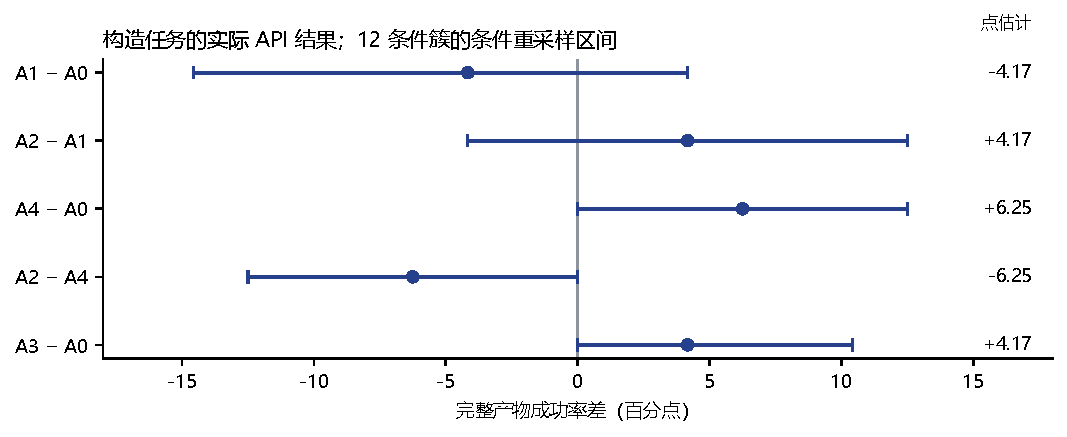
\includegraphics[width=.88\textwidth]{figures/paired_effects.pdf}
\caption{预先固定的五个配对比较。每个点来自实际API产物；线段为选定12个构造条件簇的95\%条件重采样区间，非标准误，也非技能总体的置信保证。图中颜色不编码显著性。}
\label{fig:effects}
\end{figure*}

\subsection{能力边界需要由失败层次刻画}
\begin{table}[t]
\caption{范围内输入规模分层。每个单元格为合格产物数/24次，两个重复不是独立任务。}\label{tab:sizes}
\centering\small
\begin{tabularx}{\columnwidth}{Xrr}
\toprule
方法 & 8行 & 48行 \\
\midrule
A0 无 Skill & 4/24 & 0/24 \\
A1 原始包 & 2/24 & 0/24 \\
A2 原包＋契约 & 4/24 & 0/24 \\
A3 无关上下文 & 6/24 & 0/24 \\
A4 仅契约 & 7/24 & 0/24 \\
\bottomrule
\end{tabularx}
\end{table}

六类明确元数据边界在五臂、两次重复下共60次处置全部合格。
与此同时，48行输入的120份范围内产物没有一份完整通过；
8行输入的120份产物只有23份合格（表\ref{tab:sizes}）。
边界处置和计算成功显然不能混成一个指标。
这些结果也不足以把8行认证为可靠能力区间，或把48行判定为绝对上限：
只观测了两个规模，且较小规模仍有较高失败率。

错误主要集中于过期记录计数：240份范围内产物中有216份在此项失败，
最大年龄错误20份、逐列空值错误10份、完整重复错误9份、行数错误4份。
这些错误计数可以重叠，不能相加后当作不同失败任务数。
即使温度为零，120个相同输入--方法的重复对中仍有7对的完整通过状态不同，
24对的产物数值不同；温度设定不是外部服务完全确定性的证明。

以一个8行普通CSV为例，基准日为2026-11-11，八条记录年龄依次为
$[7,1,31,8,31,7,1,0]$ 天，严格超过七天的记录应为3条。
同一输入的一次无Skill响应报告2条，原始包报告3条，而原包加契约报告0条。
其他字段可同时正确。
这一案例给出了可手工复核的失败机制，不能被引用定位或结构合格所弥补。

\subsection{事后测量诊断：平均检查掩盖完整任务失败}
这是在预定主分析之外进行的解释性诊断，不作为新的显著性检验。
每份范围内产物有9个输出字段及1个精确schema检查，共2,400项检查，
仅259项失败，平均检查通过率为\CheckPassRate\%。
即使只平均五个数据测量检查，通过率也有\MeasurePassRate\%，
但完整产物成功率仍仅\NormalPassRate\%。
该比例不是原项目既有质量分；它说明把多个容易条件与关键条件平均，
可以让同一批输出看起来远比实际可用程度好。

对同一批产物做发布门禁回放，全部接受会放行217份不合格产物；
全部拒绝虽无错误放行，但正确产物覆盖为零。
完整验收器门禁放行23份，按本构造真值没有错误放行。
后者是验收规则定义下的发布决定，不增加模型求解成功，也不是开放任务上的风险保证。
其价值在于显式呈现错误放行与覆盖，而非用全拒绝伪装优秀系统。

\subsection{网络侧：多样性没有自动形成完整能力覆盖}
\begin{table*}[t]
\caption{全库Fabric组的历史检索回放。既见12例不是新留出；相关性与完整集合覆盖分别计量。}\label{tab:routing}
\centering\small
\begin{tabularx}{\textwidth}{Xrrrr}
\toprule
方法 & 20例R@5 & 20例F & 既见12 R@5 & 既见12 F \\
\midrule
原顺序 & 80.00 & 55.00 & 78.47 & 58.33 \\
MMR .7 & 80.00 & 55.00 & 75.69 & 50.00 \\
原核DPP & 80.00 & 55.00 & 78.47 & 58.33 \\
残差DPP .5 & 80.00 & 55.00 & 78.47 & 58.33 \\
残差DPP 1 & 80.00 & 55.00 & 78.47 & 58.33 \\
查询覆盖 .5 & 80.83 & 55.00 & 78.47 & 50.00 \\
候选池上限 & 100.00 & 100.00 & 94.44 & 91.67 \\
\bottomrule
\end{tabularx}
\par\vspace{2pt}{\footnotesize R@5与F单位均为百分比；候选池上限使用参考标签作事后上界，不是实际选择器。}
\end{table*}

六种策略在全部192份捕获上产生1,152条选择记录。
表\ref{tab:routing}展示全库Fabric组，其余组别随数据一并提供。
基准20例中查询覆盖的平均召回从80.00\%升至80.83\%，
完整参考集合覆盖仍为55.00\%。
既见12例中，MMR的完整覆盖从58.33\%降至50.00\%，
查询覆盖也降至50.00\%；DPP类代理多数保持原结果。
这些结果不支持“增加多样性必然改善网络”的假设，也不能据此否定使用不同表示和训练模型的DSR。

基准20例的必要参考技能都在候选池中，但原前五只有55\%完整覆盖，
说明该组存在选择余地。
既见12例的池上限本身也不完整，未召回的参考能力无法靠重排补回。
由于任务均已使用、参考标签按技能名匹配且可能遗漏等价技能，
本文不把这组指标宣称为新的外部泛化或实际编排成功率。

\section{讨论与有效性威胁}
\subsection{哪些结论目前可信}
版本与来源窗口核验、受限参数契约和明确构造任务的验收，具有可直接复查的内部依据。
其中的可信性来自目标、输入、参照和反例的明确性，而不是模型品牌或论文引用数量。
三种实现路线对24个CSV参考结果一致，390项验收器诊断及代表案例手算核对，
降低了把一处实现错误误认成模型失败的风险；但它们仍共享研究者规定的任务语义。
本文没有独立人类质量标签，不能估计八维评分的MAE、人工一致性或语义支持准确率。

新产物实验的优势是把真实模型输出与独立目标连接起来，提供可反驳的失败，而不是由模型自报成功。
其限制也很明确：这是一个文本执行器，不使用Python或社区脚本。
原始技能建议运行工具，而当前条件不允许；因此结果刻画的是该工具受限条件下的文档注入效用，
不证明原技能在正常工具环境中同样低效。
一个确定性CSV求解器可以直接完成这些刚性任务，后续应将其作为工具路线的强对照，
而不能把“用确定性工具解决计数”包装成新颖算法。

\subsection{组合方法的增量与尚未成立的优势}
本协议把前人的多维评审、原子证据、可执行验收与集合选择连接为一个可审计流程。
实证支持的增量是：发现某些卡片参数名检查会漏掉的机械错误，
把模型提出的引用绑定到受控来源，并避免把范围外处置与完整产物成功混合报告。
标准库强对照同样检出构造错误，原包加契约未建立稳定产物优势，网络代理重排也没有普遍改善。
这些负结果限定了当前主张，不应被“更多维度”“更多反思”或“更复杂网络”取代。

仅契约组在本开发设计中使用较少上下文，并取得最高的观察成功数。
这提示后续可研究面向任务的精炼操作约束，但它不是证明简短技能总是更好。
需要扩大目标技能数、任务类型和模型，并在结果产生前固定比较与预算。
若最终只发现便宜的确定性工具已足够，应优先采用工具，而不是为了展示智能体复杂性增加开销。

\subsection{来源、任务与模型的外推限制}
D1只覆盖两个来源；原始1,881对象也不是1,881个独立仓库。
补充冻结的51个外部候选文档有5个与旧内容连接，按原仓库来源与近重关系联合分组规则，
两个新仓库都与旧来源相连，不能直接得到独立外部测试。
现有D2中的卡片混入问题仍需修正；数量凑足也不等于代表性足够。

12个新构造条件刻意包含CSV和日期陷阱，不代表真实用户任务的发生频率。
它们是开发条件，答案由研究者构造并对模型隐藏，不是独立专家认可的公开基准。
五臂、两次重复不能当作300个独立任务。
单一模型别名可能随服务更新；关闭思考和没有工具也限制结论。
因此，本文的条件区间描述该设计中的变动，不构成跨来源、跨模型或未来请求的保证。

\subsection{下一阶段的可检验路线}
第一，建立真实双盲语义标注和仲裁，比较发表版SkillNet、SkillCT画像估计、
同材料普通Judge及证据约束方法，并披露仲裁前一致性与未知比例。
第二，在合格隔离环境中允许真实工具，使用新的输入和独立产物验收，
比较无技能、原始包、精炼契约和确定性工具路线。
第三，只有单技能证据的效度得到验证后，才把它作为固定输入研究条件收益、
互补集合和验证预算分配，并检查网络更新后的旧任务遗忘\citep{P03,P06,P07,P23}。
当前研究尚不能给出经过校准的收益下界，故没有给未知节点填入任意“可信概率”。

样本量也应服从可检出效应，而不是整齐的任务数量。
假定配对不一致概率20\%、双侧阈值0.05，100个独立二元单位检测5个百分点提升的功效约14.3\%，
600个约76.0\%。
这只是规划敏感性，不是本研究观察到的效应或复杂任务族的直接功效保证。
后续需要用开发数据估计不一致率与相关性，再冻结正式留出规模。

\section{结论}
本文将开放技能包的质量核验拆成可以分别检验的证据层，
并在SkillNet-demo上完成包审查、机械干预、真实模型评价、产物对照和网络回放。
当前结果表明，接口一致、引用可定位、边界处置正确和完整产物合格之间存在实质差别。
对同一批构造任务，较高的逐项检查比例不能替代完整任务成功；
增加技能文本或集合多样性也没有自动形成稳定收益。

实际产出是可回放的核验协议、受控输入与验收器、完整失败记录、来源绑定实现及条件化结果。
它们为可靠决策提供基础，但尚未形成通用技能认证或已证明的网络优化优势。
后续工作应以独立语义参照、真实工具执行和跨来源任务验证连接这些证据层，
用真实错误放行、覆盖、产物收益和成本决定是否采用一种评价或编排方法。

\section*{数据、代码与研究状态声明}
工程与研究实现位于\url{https://github.com/qing1989620/skillnet-demo}的研究分支，草稿审查入口为
\url{https://github.com/qing1989620/skillnet-demo/pull/2}。
随稿提供LaTeX源码、44篇阅读版本的参考文献、聚合指标、300条逐次产物记录、
构造输入与答案、出图代码及构建说明。
输入、提示、模型响应、费用预留和资源指纹在本地保留不可覆盖的运行目录。
第三方完整材料、API密钥和账户总余额不进入论文数据包；第三方技能仅以固定来源与必要摘录说明。

本文是中文研究稿，未宣称获得期刊接收或同行评审认可。
文献学习为针对方法、实验和局限的定向综述，不宣称逐字通读全部正文或完成系统性元分析。
研究方案、代码分析和论文写作使用了AI辅助；被测模型输出只作为实验数据，
不充当独立人类评价者。正式投稿前仍须由项目负责人核实作者身份、机构、伦理与目标期刊要求。

\bibliographystyle{cas-model2-names}
\bibliography{references}
\clearpage
\appendix
\section{逐次结果与复现补充}
图\ref{fig:matrix}显示全部48个范围内输入--重复单元在五臂的二元结果。
每四行对应一个构造条件，包含两个输入规模及两次重复；灰色不合格项没有被删除或最佳重试替换。
逐次JSON记录还保留失败字段、实际输入输出token和响应指纹。

\begin{figure*}[t]
\centering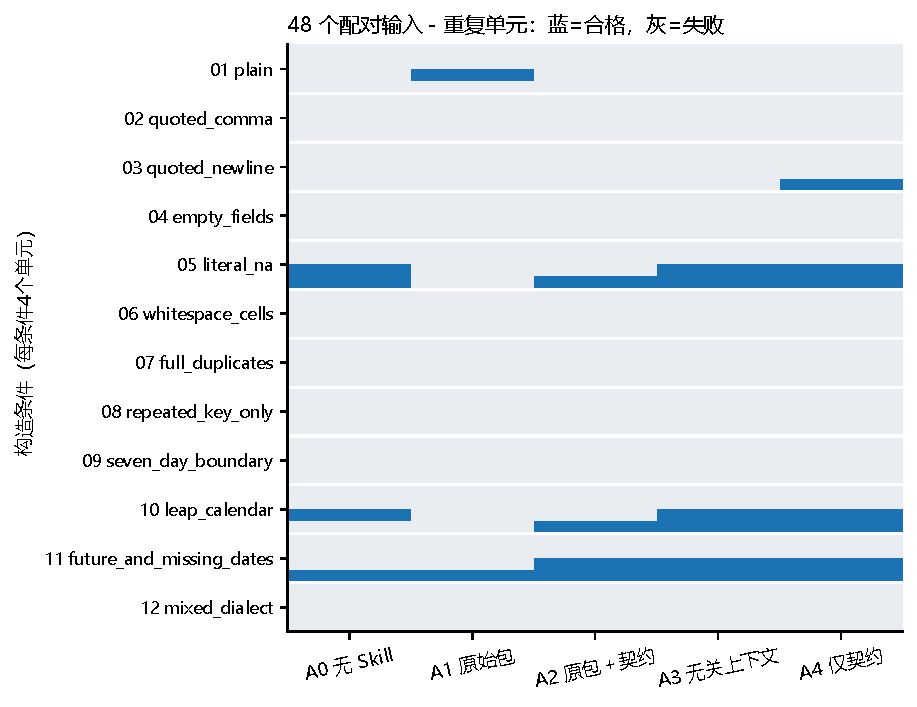
\includegraphics[width=.8\textwidth]{figures/artifact_matrix.pdf}
\caption{240份范围内实际产物的完整二元结果矩阵。数据为构造输入上的真实API输出；蓝色表示所有必需检查通过，灰色表示至少一项失败。条件排列在生成时固定，不按结果排序。}
\label{fig:matrix}
\end{figure*}

\subsection{输入与验收规则}
每个CSV包含 \texttt{id}、\texttt{amount}、\texttt{observed\_at}、\texttt{note} 四列。
构造输入的随机种子为20261111；闰年条件的基准日为2024-03-02，其余为2026-11-11。
原始记录的年龄变量保留于参考构造过程，序列化后经两个读取实现重新计算。
输入哈希由任务适配器提供供执行器复制，不把生成SHA-256作为能力测试。
每次请求是独立会话；执行器不会获得预期计数、验收代码或其他臂的答案。

对非完成状态，五个数据指标必须为空、操作列表为空，且状态须符合任务前提。
对完成状态，额外字段、缺字段、错误数值类型或任一错误指标均使完整任务失败。
这使正确格式、正确处置与正确测量分别可解释，同时防止全拒绝取得表面优胜。

\newpage
\subsection{代码与排版的验证}
新增构造任务及预算守卫通过专项检查，旧研究数据和源码指纹保留。
前期真实评价后曾修正跨平台类型标注，原始执行源码单独保存在代码快照中，
修正前后可执行语法树相同，未重复计入模型请求。
本文使用Elsevier CAS双栏类2.4和中文排版支持，由用户指定的TeX Live 2026中的XeLaTeX编译。
该模板提供版式，不代表目标期刊适配、录用状态或研究结论的权威性。

\subsection{不应从本文推出的结论}
不能将154个机械缺陷全检出写成所有技能100\%准确；
不能将来源窗口全部绑定写成语义判断全部正确；
不能将60次明确边界处置正确写成操作系统或真实二进制格式安全；
不能将观察成功数最高的方法写成跨技能、跨模型最优；
也不能将检索覆盖写成实际编排成功率。
这些限制是测量对象的一部分，而不是在结果产生后删去失败的理由。

\end{document}
